\documentclass[10pt,twocolumn,journal]{IEEEtran}
\usepackage[letterpaper, top=20mm, bottom=20mm, left=20mm, right=20mm]{geometry}
\usepackage[backend=biber,style=ieee,sorting=none]{biblatex}
\usepackage{url}
\usepackage{graphicx}
\usepackage{setspace}
\usepackage{mathptmx} % Times Roman font
\usepackage{amsmath}
\usepackage{amssymb}
\usepackage{array}
\usepackage{amstext}
\usepackage{booktabs}
\usepackage{tabularx}
\usepackage{subcaption}
\singlespacing
\addbibresource{references.bib}


\begin{document}
\title{Benchmarking LLM Architectures for Industrial Root Cause Analysis: Fine-Tuning vs. Retrieval-Augmentation}
\author{
\begin{minipage}{0.45\textwidth}
\centering
Shijun Feng\\
Product Development Unit of Packet Core Controller\\
Ericsson AB\\
\texttt{shijun.feng@ericsson.com}
\end{minipage}
\hfill
\begin{minipage}{0.45\textwidth}
\centering
Fabian Lorig\\
Department of Computer Science\\
Malmö University\\
\texttt{fabian.lorig@mau.se}
\end{minipage}
}
\maketitle
\begin{abstract}
In modern industrial software ecosystems, the high volume of operational fault reports renders manual Root Cause Analysis (RCA) a significant maintenance bottleneck, often leading to delayed resolution and high operational costs. While Large Language Models (LLMs) show promise in automating diagnostic tasks, a systematic evaluation of architectural paradigms—specifically Supervised Fine-Tuning (SFT) versus Retrieval-Augmented Generation (RAG)—remains absent in specialized industrial domains. This study presents a rigorous benchmarking of three distinct architectures: an encoder-decoder model (T5), a lightweight decoder-only baseline (GPT-2), and a RAG framework, evaluated on a curated dataset of real-world industrial fault reports. Our findings reveal a critical architectural trade-off: $T5$ achieves superior lexical and structural fidelity (e.g., BLEU-4 of 0.1810 vs. GPT-2’s 0.1210), whereas RAG provides the highest semantic alignment (BERTScore of 0.7715). These results suggest that while SFT is optimal for generating structured reports, RAG is superior for contextually grounded reasoning in complex fault scenarios. We propose a hybrid framework that leverages the structural precision of T5 and the semantic depth of RAG, providing a metric-driven roadmap for deploying intelligent RCA assistants in industrial software maintenance workflows.
\end{abstract}

\begin{IEEEkeywords}
Root Cause Analysis (RCA), Large Language Models (LLM), T5, GPT-2, Retrieval-Augmented Generation (RAG), Software Maintenance, Fine-tuning.
\end{IEEEkeywords}

\section{INTRODUCTION}
\label{sec:introduction}

Modern cloud-native networks generate a high volume of operational trouble reports, making Root Cause Analysis (RCA) a significant maintenance bottleneck. Currently, fault report management is largely manual and experience-driven, leading to delayed response times and redundant work—particularly in identifying duplicate issues across diverse environments Pedroso et al. \cite{10979844}. The lack of automated frameworks increases the risk of inconsistent handling and human error in correlating system behaviors and logs Afshinpour et al. \cite{10684586}.

While Large Language Models (LLMs) have shown potential in automating software engineering tasks Chen et al. \cite{chen2024automatic}, Han et al. \cite{10765066}, existing studies often evaluate models in isolation. There is a lack of systematic comparison between architectural paradigms—specifically supervised fine-tuning (SFT) versus retrieval-augmentation—within specialized industrial domains. This study addresses this gap by benchmarking three distinct architectures: a fine-tuned encoder-decoder model (T5), a decoder-only autoregressive model (GPT-2), and a Retrieval-Augmented Generation (RAG) system using a curated dataset of textual fault reports.

The primary contributions of this paper are:
\begin{itemize}
    \item Performance Evaluation: A quantitative analysis of Fine-Tuning T5 and GPT-2 models using lexical (BLEU, ROUGE) and semantic (BERTScore) metrics.
    \item Architectural Comparison: A side-by-side comparison of SFT versus RAG approaches, identifying trade-offs in output quality and engineering workflow alignment.
    \item Selection Framework: A metric-driven framework to guide practitioners in selecting or hybridizing LLM architectures for industrial RCA tasks.
\end{itemize}

The remainder of this paper is structured as follows: Section \ref{sec:research-questions} formulates the research questions guiding this benchmarking study; Section \ref{sec:related-work} surveys existing approaches to automated RCA and positions this work within the broader LLM landscape; Section \ref{sec:methodology} describes the experimental design, dataset preparation, and evaluation metrics; Section \ref{sec:results} presents a detailed quantitative analysis comparing the three architectures; Section \ref{sec:threats} discusses potential threats to validity; and Section \ref{sec:conclusion} summarizes key findings and outlines future research directions.

\section{RESEARCH QUESTIONS}
\label{sec:research-questions}

To address the challenges of automating software diagnostic reporting, this study investigates the following research questions:

\begin{itemize}
    \item RQ1: To what extent can Large Language Models (LLMs) be Fine-Tuning on domain-specific fault report data to generate lexically and semantically accurate RCA explanations?
    \item RQ2: How do supervised Fine-Tuning (SFT) architectures (e.g., T5, GPT-2) compare to Retrieval-Augmented Generation (RAG) paradigms regarding output quality and alignment with engineering workflows?
    \item RQ3: How do the computational overhead and the requirement for domain-specific grounding influence the choice between SFT and RAG for industrial software maintenance?
\end{itemize}

Consistent with the technical scope of this study, model performance is evaluated exclusively through automated Natural Language Generation (NLG) metrics, specifically BLEU, ROUGE, and BERTScore. While human-centric evaluation (e.g., expert-rated utility) is recognized as a vital component of practical deployment, it remains outside the scope of this baseline quantitative assessment.

\section{RELATED WORK}
\label{sec:related-work}
\subsubsection{Traditional ML Approaches in RCA}
Root cause analysis (RCA) using machine learning has gained significant traction across domains such as software engineering, manufacturing, and networking. Traditional approaches often apply supervised models like support vector machines (SVMs), decision trees, or Naïve Bayes classifiers to classify faults based on historical data.

Wang et al. \cite{wang2021rootcause} train SVMs on textual bug reports to predict fault types (e.g., concurrency, memory, semantic bugs), achieving solid accuracy but providing no interpretability or semantic insight to support engineers during resolution. Chen et al. \cite{chen2017pca} combine PCA and SVM for fault detection in manufacturing, successfully identifying key structured features but excluding natural language inputs. Similarly, Zhang et al. \cite{zhang2022sdn} apply ML to SDN faults using time-series data, offering fast classification but limited diagnostic support.

Among interpretable models, Jovic et al. \cite{jovic2023naivebayes} use Naïve Bayes to identify predictive terms in bug descriptions, offering limited lexical guidance to engineers. However, none of these works integrate semantic retrieval or lexical pattern analysis to directly aid fault resolution.

\subsubsection{Neural Network and Deep Learning Approaches in RCA}
Deep learning has been increasingly adopted for root cause analysis (RCA), particularly in domains like manufacturing, network management, and software systems. Unlike traditional machine learning approaches, deep neural networks offer powerful feature learning capabilities, but not all methods provide semantic insight or lexical interpretability needed to support engineers in resolving issues.

Artificial neural networks (ANNs) and residual causal models like Sparse Causal Residual Neural Networks (SCRNN) have been applied to structured sensor data in manufacturing and quality control tasks Chen et al. \cite{chen2022scrnn}. These models perform well in predicting fault contributors from numerical logs but do not operate on natural language input or offer semantic interpretability.

Other approaches leverage deep learning architectures such as convolutional neural networks (CNNs), recurrent neural networks (RNNs), autoencoders, and transformers for unsupervised anomaly detection in system logs Singh et al. \cite{anomaly2021dl}. While these methods are useful for identifying outliers, they typically lack causal reasoning and are not designed to interpret textual summaries or aid fault resolution.

More promising results are seen in graph-based models. KGroot Zhao et al. \cite{kgroot2024}, a recent framework combining knowledge graphs with graph convolutional networks (GCNs), constructs semantic fault graphs from event traces and textual logs. It enables similarity-based retrieval of past faults with known causes, providing contextual and semantic guidance. This makes it particularly well-suited for cases where fault descriptions, priorities, and summaries are available.

Another technique involves combining LSTM networks with Bayesian neural networks (BNNs) to model probabilistic causality across time-series data Li et al. \cite{lstm2023bnn}. Though effective in capturing causal structures, it relies entirely on structured logs and does not process natural language input.
\subsubsection*{Summary of Related Work}
Traditional machine learning and deep learning methods have laid the foundation for automated root cause analysis, especially in classification and clustering tasks. However, these approaches often fall short in dealing with unstructured, domain-specific text where lexical and semantic nuance is crucial. Recent work using graph-based or retrieval-augmented models has improved case similarity detection, yet lacks generalization across diverse linguistic expressions. This opens the door for large language models (LLMs), which inherently support contextual understanding, semantic retrieval, and natural language generation. As such, this study explores whether LLMs—specifically T5, GPT-2, and RAG—can serve not as replacements but as intelligent assistants to engineers performing RCA, addressing both relevance and clarity in fault resolution.

\section{METHODOLOGY}
\label{sec:methodology}

This section details the research methodology, experimental setup, data preparation, and evaluation procedures used to compare the performance of Large Language Models (LLMs) in generating Root Cause Analysis (RCA) explanations.

\subsection{Research Approach and Scope}
\label{sec:research-approach}

The study employs a quantitative, experimental, and comparative methodology rooted in a positivist paradigm. The objective is the objective, measurable, and replicable evaluation of different LLM architectures for RCA tasks. We utilize an experimental design to assess model outputs under controlled conditions using standardized, automated metrics (BLEU, ROUGE, BERTScore).

The research is strictly limited to textual input features (Summary, Description, Priority, Answer) and automated evaluation metrics, focusing on establishing a technical baseline for language-based RCA capabilities.

\subsection{Data Source and Preprocessing}
\label{sec:data-preprocessing}

\subsubsection{Data Source and Ethics}
The dataset consists of 6,582 historical fault reports sourced from Ericsson's internal Jira system. Each report includes structured metadata and unstructured text. In compliance with internal data governance and Data Protection Officer (DPO) approval, all personal identifiers and columns (e.g., author names, comments) were removed to ensure anonymity and data security. All experiments were conducted within a secure corporate intranet environment.

\subsubsection{Feature Selection and Ground Truth}
The final dataset utilized four key fields. The expert-written RCA serves as the Ground Truth (Target Variable).
\begin{itemize}
    \item Input Features: Summary, Description, and Priority (Importance Code).
    \item Target Feature (Ground Truth): Answer (the expert-written RCA).
\end{itemize}
The Answer field follows a standardized, multi-component structure, including the Condition, Description of fault, and Correction (See Table \ref{tab:answer-structure}).

\begin{table}[ht]
\centering
\caption{Standardized Answer Structure for RCA (Root Cause Analysis)}
\label{tab:answer-structure}
\begin{tabularx}{\columnwidth}{>{\bfseries}p{0.25\columnwidth} >{\raggedright\arraybackslash}X }
\toprule
Component & Function in RCA \\
\midrule
Condition & Description of conditions that trigger the fault. \\
\\
Description of the fault & Detailed technical explanation of the issue. \\
\\
Description of the correction & The steps taken or planned to resolve the fault. \\
\bottomrule
\end{tabularx}
\vspace{1em}
\end{table}

\subsubsection{Data Cleaning and Wrangling}
The raw data underwent several preprocessing steps:
\begin{enumerate}
    \item Consolidation: Fault reports pointing to the same underlying resolution were grouped to prevent treating duplicates as independent training samples.
    \item Null Handling: Entries lacking a value in the critical Answer column were removed.
    \item Partitioning: The cleaned dataset was randomly partitioned into a Training set (80\%) and a Validation set (20\%), stratified by Priority.
\end{enumerate}

\subsection{Model Architectures and Implementation}
\label{subsec:model_architectures}

To evaluate the trade-offs between different architectural paradigms for industrial RCA, we implemented three models representing state-of-the-art sequence-to-sequence learning, autoregressive generation, and retrieval-augmented reasoning. All experiments were conducted using the Hugging Face Transformers library within a containerized Kubeflow environment.

\subsubsection{Supervised Fine-Tuning (SFT) Architectures}
We selected two models to evaluate the impact of architectural directionality on RCA generation:
\begin{itemize}
    \item T5-Small: An encoder-decoder (Seq2Seq) model with approximately 60 million parameters. T5 was chosen for its unified ``text-to-text'' framework, which is optimized for conditional generation tasks where the output must conform to a rigid structural template.
    \item GPT-2 (Base): A decoder-only autoregressive model with 124 million parameters. This serves as a baseline to evaluate how unidirectional context handles the causal relationship between fault descriptions and resolutions.
\end{itemize}

\subsubsection{Retrieval-Augmented Generation (RAG) Architecture}
The RAG framework was implemented to ground the model's outputs in historical context, mitigating the risk of neural hallucinations in technical diagnostics.

\begin{itemize}
    \item Dense Passage Retrieval (DPR): We used the\\
    \texttt{facebook/dpr-question\_encoder-single- \\
    nq-base} encoder to encode fault reports into dense
    768-dimensional vectors. 
    \item Retrieval Logic: For a given query report $q$, the system calculates the cosine similarity against a pre-computed corpus tensor of historical resolutions. The retriever identifies the top $k=5$ most relevant contexts, which are then concatenated with the input prompt to provide the generative component with domain-specific grounding.
\end{itemize}

\subsubsection{Training Protocols and Hyperparameters}
The SFT models were fine-tuned for 10 epochs using the AdamW optimizer with a weight decay of 0.01. To ensure a fair comparison, we standardized the following hyperparameters:
\begin{itemize}
    \item Learning Rate: $5 \times 10^{-5}$ with a linear warmup.
    \item Sequence Length: Max input and output length set to 512 tokens, utilizing truncation for long technical logs.
    \item Hardware: Training was executed on a single NVIDIA GPU (16 GB VRAM) with 30 GB of system RAM.
    \item Regularization: Early stopping was triggered if the validation loss failed to improve for three consecutive epochs to prevent overfitting to customer-specific patterns.
\end{itemize}
% \subsection{Model Architectures and Setup}
% \label{sec:model-arch}

% Three distinct LLM architectures were selected to represent different paradigms in text generation relevant to RCA.

% \begin{table}[ht]
% \centering\small
% \caption{Summary of Model Architectures}
% \label{tab:models-summary}
% % The column widths are adjusted:
% % Column 1: Fixed 15% width (p{0.15\columnwidth})
% % Column 2: Fixed 25% width (p{0.25\columnwidth})
% % Column 3: The rest (X), now ~60%
% \begin{tabularx}{\columnwidth}{
%     >{\bfseries}p{0.15\columnwidth} 
%     >{\raggedright}p{0.25\columnwidth} 
%     >{\raggedright\arraybackslash}X 
% }
%     \toprule
%     Model & Type & Rationale for RCA \\
% \midrule
% T5 (Base) & Encoder-Decoder (Seq2Seq) & Unified Text-to-Text transformation for structured output. \\
% \\
% GPT-2 (Medium) & Autoregressive Decoder & Evaluates flexible, free-form generative capabilities. \\
% \\
% RAG & Retrieval-Augmented & Evaluates benefit of external grounding via historical context. \\
% \bottomrule
% \end{tabularx}
% \end{table}
% \subsubsection{Training Environment}
% Experiments were executed in a containerized Kubeflow environment using Python, the Hugging Face Transformers library, and PyTorch. The hardware setup included 1 GPU (16 GB memory) and $\sim$30 GB RAM.

% \subsubsection{Model Training and Hyperparameters}
% The T5 and GPT-2 models were fine-tuned on the Training set. Key hyperparameters included setting the Max Input/Output Sequence Length to 512 tokens. Training was performed for up to 10 epochs using the AdamW optimizer with early stopping based on validation loss to prevent overfitting.

\subsection{Evaluation Metrics and Procedure}
\label{sec:evaluation}
Model performance was assessed using a combination of automated Natural Language Generation (NLG) metrics against the expert-written Ground Truth:
\begin{itemize}
    \item BLEU: Measures lexical fidelity and precision based on n-gram overlap.
    \item ROUGE: Measures completeness and recall, focusing on unigram (ROUGE-1) and Longest Common Subsequence (ROUGE-L) overlap.
    \item BERTScore: Measures semantic similarity by computing the cosine similarity between contextual embeddings, accounting for meaning beyond exact word matches.
\end{itemize}


The Evaluation Procedure involved generating an RCA for every entry in the 20\% Validation set and computing the three metric scores (BLEU, ROUGE, BERTScore) against the reserved Ground Truth answers.
% (duplicate line removed - use previous line with texttt formatting)

\section{RESULTS AND DISCUSSION}
\label{sec:results}

This section presents the quantitative evaluation of the three model architectures: T5, GPT-2, and RAG. Performance is assessed on the 20\% validation set using standard Natural Language Generation (NLG) metrics.

\subsection{Training Dynamics Analysis}

The fine-tuning process for the generative models (T5 and GPT-2) was monitored to assess stability and generalization.

\begin{itemize}
    \item T5 Performance: The T5 model exhibited minor fluctuations in training loss but maintained a stable validation loss throughout all 10 epochs. This stability indicates that the Encoder-Decoder architecture generalized effectively to the unseen fault report data.
    \item GPT-2 Performance: The GPT-2 model showed significant instability and erratic fluctuation in training loss (ranging between 1.67 and 3.00). This inconsistent convergence suggests that the autoregressive, decoder-only architecture struggled to adapt to the structured, sequence-to-sequence nature of the RCA task.
\end{itemize}
The performance of the RAG model is evaluated primarily through its end-to-end output metrics in Section \ref{sec:quantitative-comparison}, as generation loss alone does not fully capture its effectiveness.

\begin{figure}[h!]
    \centering
    \begin{subfigure}[b]{0.48\textwidth}
        \centering
        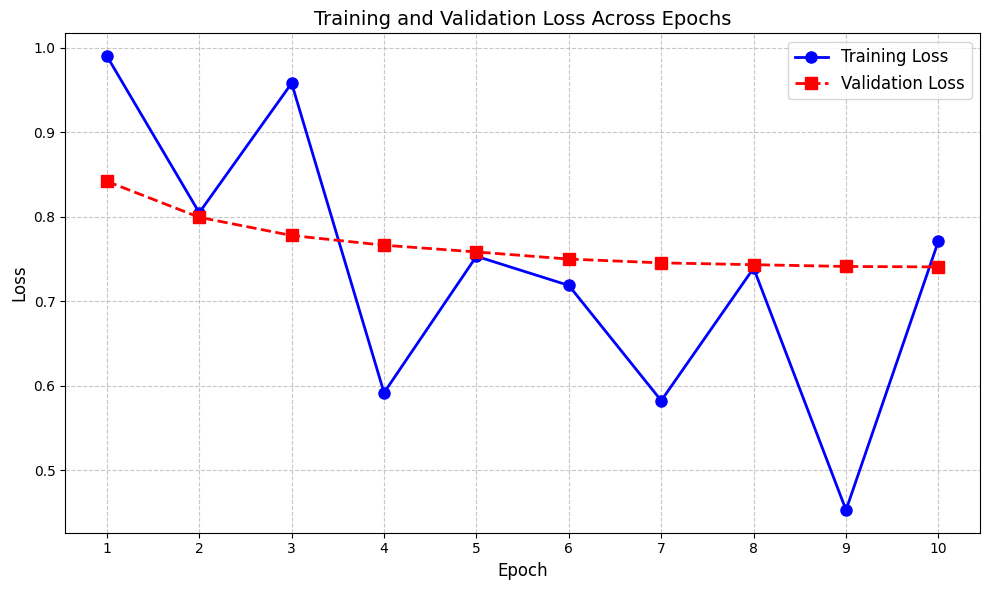
\includegraphics[width=\linewidth]{image/t5-small-training.png}
        \vspace{-0.3cm}
        \caption{T5 Training \& Validation Loss}
    \end{subfigure}
    \hfill
    \begin{subfigure}[b]{0.48\textwidth}
        \centering
        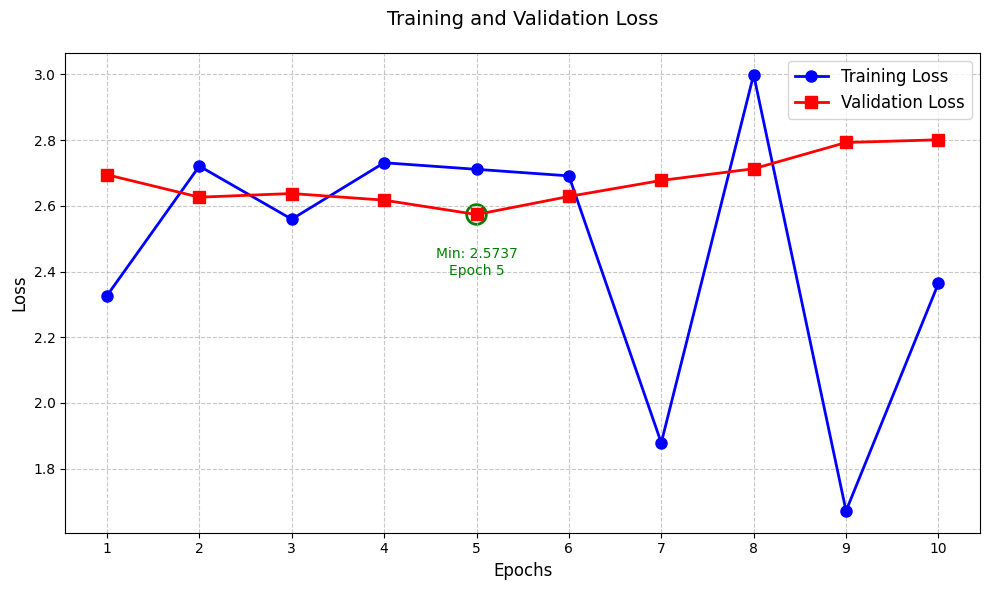
\includegraphics[width=\linewidth]{image/gpt2-training-validation-loss.png}
        \vspace{-0.3cm}
        \caption{GPT-2 Training \& Validation Loss}
    \end{subfigure}
    \caption{T5 and GPT-2 Training and Validation Loss Curves}
    % \Description{Training and validation loss curves for T5 and GPT-2 models}
\end{figure}

\subsection{Quantitative Metric Comparison}
\label{sec:quantitative-comparison}

The models were evaluated by comparing their generated RCA explanations against the expert-written ground truth using lexical overlap metrics (BLEU, ROUGE) and semantic similarity (BERTScore). The results are summarized in Table \ref{tab:model_comparison}.
\begin{table}[h]
\raggedright
\footnotesize
\caption{Model Performance Comparison on RCA Generation}
\label{tab:model_comparison}
\begin{tabularx}{\columnwidth}{X c c c c c}
\toprule
Model  & BLEU & R-1 & R-L & R-2 & BERT \\
\midrule
T5 & 0.1810 & 0.3869 & 0.3463 & 0.2821 & 0.5478 \\
GPT-2 & 0.1210 & 0.1885 & 0.1001 & 0.0432 & 0.4674 \\
RAG & 0.0037 & 0.0682 & 0.0447 & 0.0072 & 0.7715 \\
\bottomrule
\end{tabularx}
\end{table}

\subsubsection{Lexical and Structural Fidelity}
The T5 model achieved the highest scores across all lexical metrics (BLEU-4, ROUGE-1, ROUGE-L, ROUGE-2). This demonstrates its ability to reproduce the specific terminology and structured format required for formal RCA documentation. The RAG model recorded the lowest lexical scores (BLEU-4=0.0037), reflecting its tendency to paraphrase retrieved information rather than matching exact n-grams from the ground truth.

\subsubsection{Semantic Similarity}
The RAG model achieved the highest semantic similarity score (BERTScore=0.7715). Since BERTScore evaluates meaning beyond exact word matches, this finding is crucial: the RAG model generates contextually and technically equivalent explanations, highlighting its strength in knowledge grounding. The T5 model's BERTScore of 0.5478 confirmed a strong balance between structured output and semantic correctness.

\subsubsection{Metric Sensitivity and Architectural Divergence}
A notable discrepancy is observed in the RAG model's performance, which recorded a near-zero BLEU-4 score (0.0037) despite achieving the highest BERTScore (0.7715). This divergence highlights the limitations of n-gram-based metrics for retrieval-based systems. While T5 is optimized to minimize cross-entropy loss against a specific ground-truth string (leading to high lexical fidelity), the RAG model synthesizes information from historical contexts that may be semantically identical but linguistically distinct from the target answer. The high BERTScore confirms that the RAG model captures the technical essence of the fault resolution, even when it does not mimic the exact phrasing of the original engineer.

\subsection{Synthesis of Findings and Proposed Selection Framework}
\label{sec:synthesis}

The evaluation demonstrates a distinct trade-off in architectural performance for RCA. Our quantitative analysis reveals that T5 excels in structured reporting and automation, achieving the highest lexical scores necessary for outputs that conform to rigid documentation standards. Specifically, T5 attained a BLEU-4 of 0.1810. Conversely, the RAG architecture demonstrated superior semantic relevance and reasoning, achieving the highest BERTScore of 0.7715, which is critical for providing contextually-grounded insights. 

These results provide the quantitative basis for guiding the selection of LLM architectures in industrial workflows. To resolve the observed performance gap between lexical precision and semantic depth, we propose a hybrid RAG-T5 architectural framework, as illustrated in Fig. 2.

\begin{figure}[htbp]
    \hspace*{-10mm}\centering
    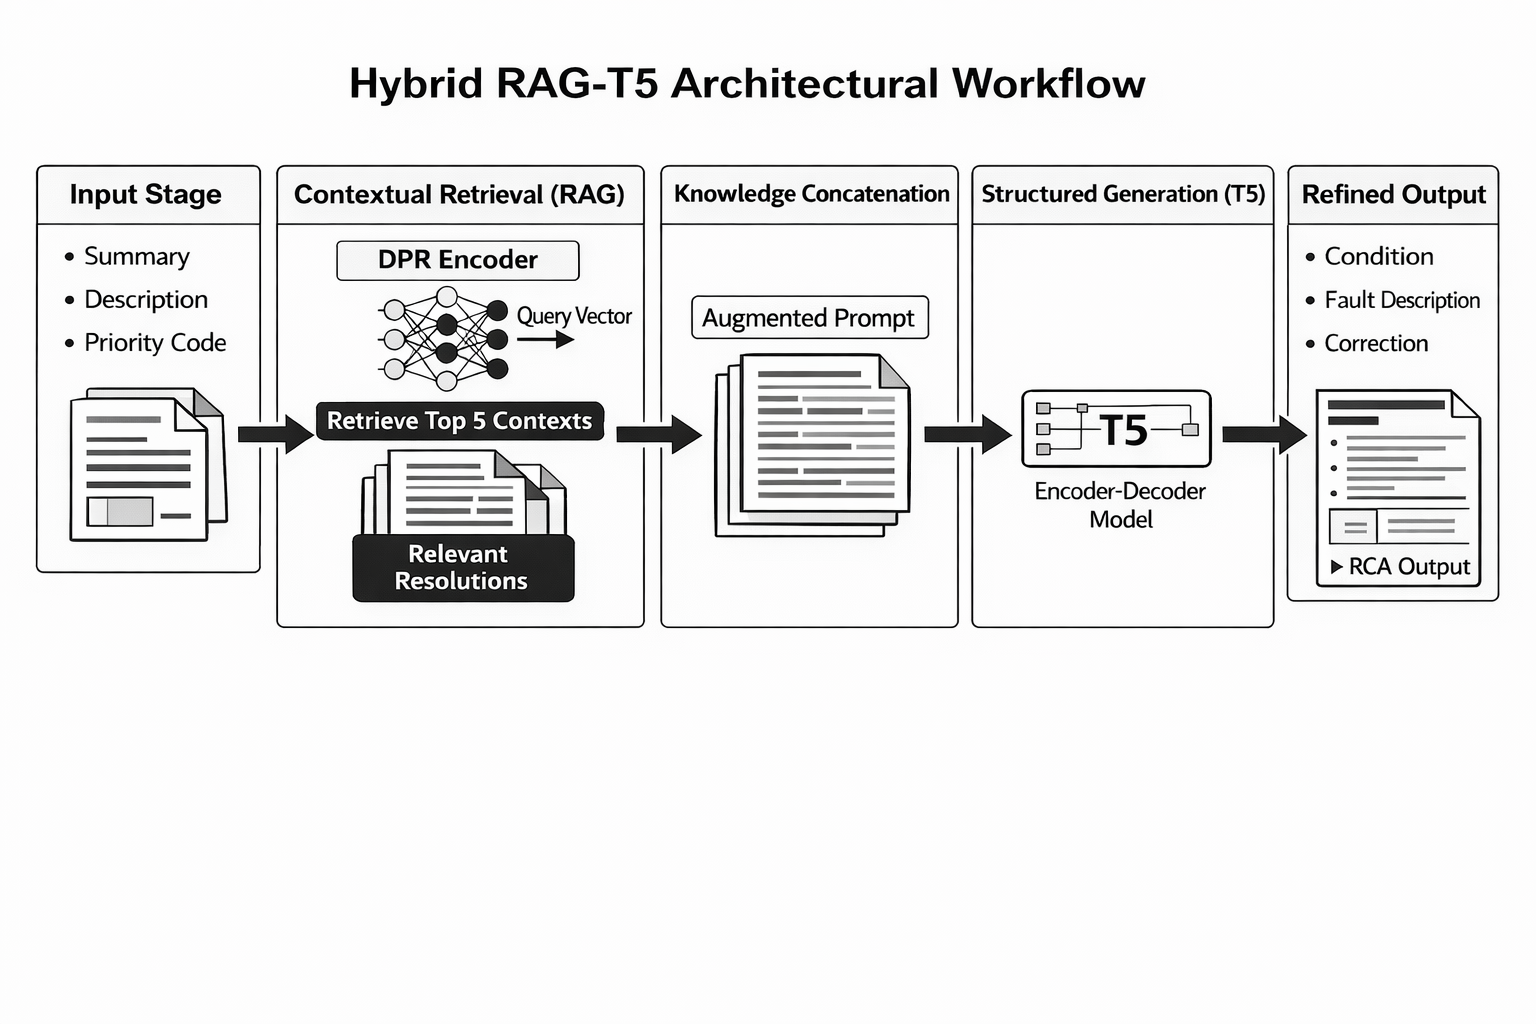
\includegraphics[width=0.55\textwidth]{image/RAG-T5.png}
    \caption{Proposed Hybrid RAG-T5 Framework: Integrating historical retrieval grounding for semantic depth with T5 generative decoding for structural fidelity.}
    \label{fig:hybrid-framework}
\end{figure}

The proposed framework leverages the structural precision of T5 and the semantic depth of RAG to provide a metric-driven roadmap for industrial maintenance. It functions in two primary stages:
\begin{enumerate}
    \item Contextual Grounding: A retrieval component (DPR) identifies the top $k=5$ historical resolutions to ensure technical accuracy and minimize hallucinations.
    \item Structural Synthesis: The retrieved context is processed by a fine-tuned T5 model to ensure the output conforms to the standardized three-part RCA template (Condition, Description, and Correction).
\end{enumerate}

This hybridization is identified as the most robust strategy for balancing documentation requirements with the interpretive value needed by human engineers.

% \subsection{Synthesis of Findings}
% The evaluation demonstrates a distinct trade-off in architectural performance for RCA:
% \begin{itemize}
%     \item T5 excels in structured reporting and automation, achieving the highest lexical scores necessary for outputs that conform to rigid documentation standards.
%     \item RAG excels in semantic relevance and reasoning, achieving the highest $\text{BERTScore}$ which is critical for providing deep, contextually-grounded insights valuable to a human engineer.
% \end{itemize}
% These results provide the quantitative basis for guiding the selection of LLM architectures in practical engineering workflows.

\section{Threats to Validity}
\label{sec:threats}

While our findings provide a benchmark for LLM-based RCA, several factors may influence the generalizability and robustness of the results.

\subsection{Internal Validity}
Internal threats relate to the quality of the ground truth and model training. The expert-written resolutions in the Jira dataset occasionally exhibit varying levels of detail, which introduces noise into the training signal. Furthermore, while the T5 and GPT-2 models were fine-tuned until loss convergence, the stochastic nature of neural generation implies that different random seeds or hyperparameter configurations could yield marginal variations in lexical scores. We mitigated this by utilizing standardized protocols and early stopping.

\subsection{External Validity}
External threats concern the generalizability of our findings. This study was conducted using a dataset specific to a single industrial domain (telecommunications). Consequently, the performance of the DPR-based RAG and the fine-tuned T5 model may vary when applied to software systems with different logging formats or resolution styles. However, the architectural trade-offs identified (lexical vs. semantic priority) are likely consistent across diverse industrial RCA tasks.

\subsection{Construct Validity}
Construct threats involve the suitability of our evaluation metrics. We utilized BLEU and ROUGE to measure lexical overlap; however, these metrics do not always correlate with human-perceived utility in a diagnostic context. While we addressed this by incorporating BERTScore to measure semantic similarity, a remaining threat is the absence of a qualitative human-in-the-loop study. Future work will include expert-led evaluations to bridge the gap between automated metrics and real-world engineering value.

\section{CONCLUSION AND FUTURE WORK}
\label{sec:conclusion}

This study investigated the application of Large Language Models (LLMs) for automated Root Cause Analysis (RCA) in software fault reports, comparing Fine-Tuning generative models (T5, GPT-2) with a Retrieval-Augmented Generation (RAG) approach.

\subsection{Summary of Findings}
The experimental results provide several key insights:
\begin{itemize}
    \item Architectural Performance: Fine-tuning domain-specific LLMs significantly enhances diagnostic accuracy. T5 emerged as the superior model for structured reporting, achieving the highest lexical fidelity. Conversely, RAG demonstrated superior semantic alignment. This suggests that lexical metrics like BLEU may penalize RAG systems for generative creativity, whereas semantic metrics like BERTScore more accurately reflect their utility in providing diverse yet technically sound diagnostic insights.
    \item Metric-Driven Evaluation: Automated metrics successfully captured complementary aspects of model performance. While BLEU and ROUGE identified the structural strengths of T5, BERTScore highlighted the interpretive value of RAG, establishing a systematic foundation for evaluating RCA tasks without immediate human intervention.
    \item Selection Framework: We introduced a three-dimensional framework—comprising Output Quality, Domain Alignment, and Usability—to guide model selection. The analysis indicates that a hybrid RAG-T5 approach is likely the most robust strategy for balancing structural documentation requirements with semantic precision.
\end{itemize}



\subsection{Contributions and Limitations}
This research establishes a replicable baseline for LLM-based RCA in software engineering. However, the study's scope was constrained by: (i) an exclusive focus on textual data, omitting multimodal diagnostic signals such as logs and charts; (ii) inherent noise in the expert-written ground truth labels; and (iii) the use of automated metrics as a proxy for human expert judgment. Despite these constraints, the study demonstrates that domain-specific fine-tuning makes LLM integration feasible for real-world fault management.

\subsection{Future Work}
Future research will build upon this foundation in the following directions:
\begin{itemize}
    \item Hybrid Prototype Development: Implementing an integrated RCA assistant that combines RAG's retrieval capabilities with T5's generation quality to support interactive engineering workflows.
    \item Multimodal Integration: Extending model architectures to process heterogeneous data sources, including system logs, performance metrics, and commit histories, to improve diagnostic depth.
    \item Human-in-the-Loop Validation: Conducting qualitative studies with domain experts to assess the interpretability, trust, and practical usability of model-generated RCA explanations.
    \item Scalability and Generalization: Evaluating larger model variants (e.g., T5-Large, GPT-4) across diverse industrial datasets to mitigate training instabilities and enhance cross-domain generalization.
\end{itemize}
\printbibliography
\end{document}